\documentclass[12pt]{article}
\usepackage[a4paper, bindingoffset=0.2in, %
							left=0.5in,right=0.5in,top=0.5in,bottom=0.5in,%
							footskip=.25in]{geometry}
\usepackage{graphicx}
\usepackage{listings}
\usepackage{amssymb}
\usepackage{hyperref}

\title{PSet1 Report}
\author{Ali Abolhassanzadeh Mahani}
\date{Sep. 28}

\begin{document}
    \maketitle
    \section{Problem 1}
    \subsection{Creations and the loops}
    For starters, since I know how many steps I'm going to have and the size of the row,
    I allocate a table of that size in memory using \texttt{np.ndarray} with \texttt{int} as my data type; This will be my canvas.
    
    Now,  I do a nested for loop for each \textit{round} and each \textit{element} in the row
    to find their situation and decide their next state. Here, some people use 
    \texttt{(index) \% len(row)} to set the boundary condition, but with this setup, we are doing a \texttt{mod operation} per element and it makes it a little inefficient. I used the fact that Python \texttt{ndarray}s support \emph{negative indexing} and just set the upper boundary condition with an if statement.
    
    \subsection{The rule}
    Our rule is as follows: \emph{``If \underline{only one} of my neighbors is 1 (i.e. Has a hat), I become 1 (i.e. put on the hat), otherwise, I become 0."}
    
    The mathematical interpretation of \emph{``If only 1 neighbor is 1"} is that the sum of the neighbors equals to 1. Hence the \texttt{if} statement in our code.
    
    \subsection{Fancy}
    The style of which I have written this code is to be able to import the functions, if I
    need them in the future. All that the last \texttt{if} statement does, is to see if we are executing this file, and then, execute the \texttt{main()} function.
    
    \subsection{Analysis} \label{sec:analysis}
    The main part of the code is the \texttt{put\_hat()} function, which consists mainly of two
    nested \texttt{for} loops. taking one to have $m$ iterations and the other, $n$, we can see 
    that the runtime complexity of this code is $\mathcal{O}(m.n)$.
    In order to analyze this code, one can run a profiler on it as follows:
    \begin{lstlisting}[language=bash]
    	python -m cProfile -s time Hats.py
    \end{lstlisting}
	Note that this profiler lists all the modules that are being called, so due to our use of \texttt{numpy} and \texttt{matplotlib.pyplot}, it will show a lot of things, but the main 
	function \texttt{put\_hats} will be at the top few.
    
	
	\subsection{Results}
	I used the \texttt{pcolormesh()} module from the \texttt{matplotlib.pyplot} library to
	export my canvas into a file. The resulting image is identical to rule 18, 26 or 90. (Figure \ref{fig:hats200})
	\begin{figure}[h!]
		\includegraphics[width=\linewidth]{../P1/Hats200.jpg}
		\label{fig:hats200}
		\caption{The evolution of the hats for 200 steps using the rule that if only one of
							my neighbors has a hat, I put on a hat, otherwise, I put down my hat. The yellow cells have a hat on and the purple ones don't.
							\emph{Note that this rule is independent of the item in question.}}
	\end{figure}

	\section{Problem 2}
	\subsection{The Code}
	This project consists of 3 files. \texttt{256rules.py} which is the main file to be run,
	\texttt{cells.py} which contains the creation and evolution of cells, and finally, \texttt{graphics.py} which contains the modules to make the image files.
	
	As for analysis, one can use the code used in section\ref{sec:analysis} to run a profiler on the main functions. But the algorithm used is the same as the one before.
	
	\subsection{Results}
	Using the \texttt{graphics.py} module we output the file with its rule number in binary as its name. The result are included in Fig \ref{fig:2rules}.   As one can see, the CA rule 75 makes a chaotic-looking pattern meaning that
	it's classified in \textbf{Class 3} in Wolfram, while rule 110 leads to a comples pattern that seems to repeat itself locally, hence in \textbf{Class 4} in Wolfram.
	\begin{figure}[h!]
		\includegraphics[width=0.45\linewidth]{../P2/Hats01001011.jpg}
		\includegraphics[width=0.45\linewidth]{../P2/Hats01101110.jpg}
		\label{fig:2rules}
		\caption{These images where created using rules 110 (on the right) and 75 (on the left)
							 of the 256 Elementary Cellular Automata Rules. Color yellow means the 
							 cell is \emph{on} and purple means that it's \emph{off}. }
	\end{figure}
	
	\section{Problem 3}
	\subsection{The Code}
	This project is almost identical to the previous one. The only difference is the main file
	\texttt{iteration\_bitflip.py}. This time we take rule 110 and iterate over its digits and do a
	bit flip for each one. Then we make the CA for that rule and output it as before.
	\subsection{Results}
	The result are the same as the ones in question in the assignment.
	(Figure \ref{fig:bitflip}) As one can see, rules \texttt{00101110}, \texttt{01101010}, \texttt{01101100} are Class 2 CAs and  rules \texttt{01001110}, \texttt{11101110}, \texttt{01100110} 
	are class 4 CAs, while \texttt{01101111}, \texttt{01111110} seem chaotic and are classified as Class 3 CAs.
	
	\begin{figure}[h!]
		\includegraphics[width=0.4\linewidth]{../P3/Hats00101110.jpg}
		\includegraphics[width=0.4\linewidth]{../P3/Hats01001110.jpg}
		\includegraphics[width=0.4\linewidth]{../P3/Hats01100110.jpg}
		\includegraphics[width=0.4\linewidth]{../P3/Hats01101010.jpg}
		\includegraphics[width=0.4\linewidth]{../P3/Hats01101100.jpg}
		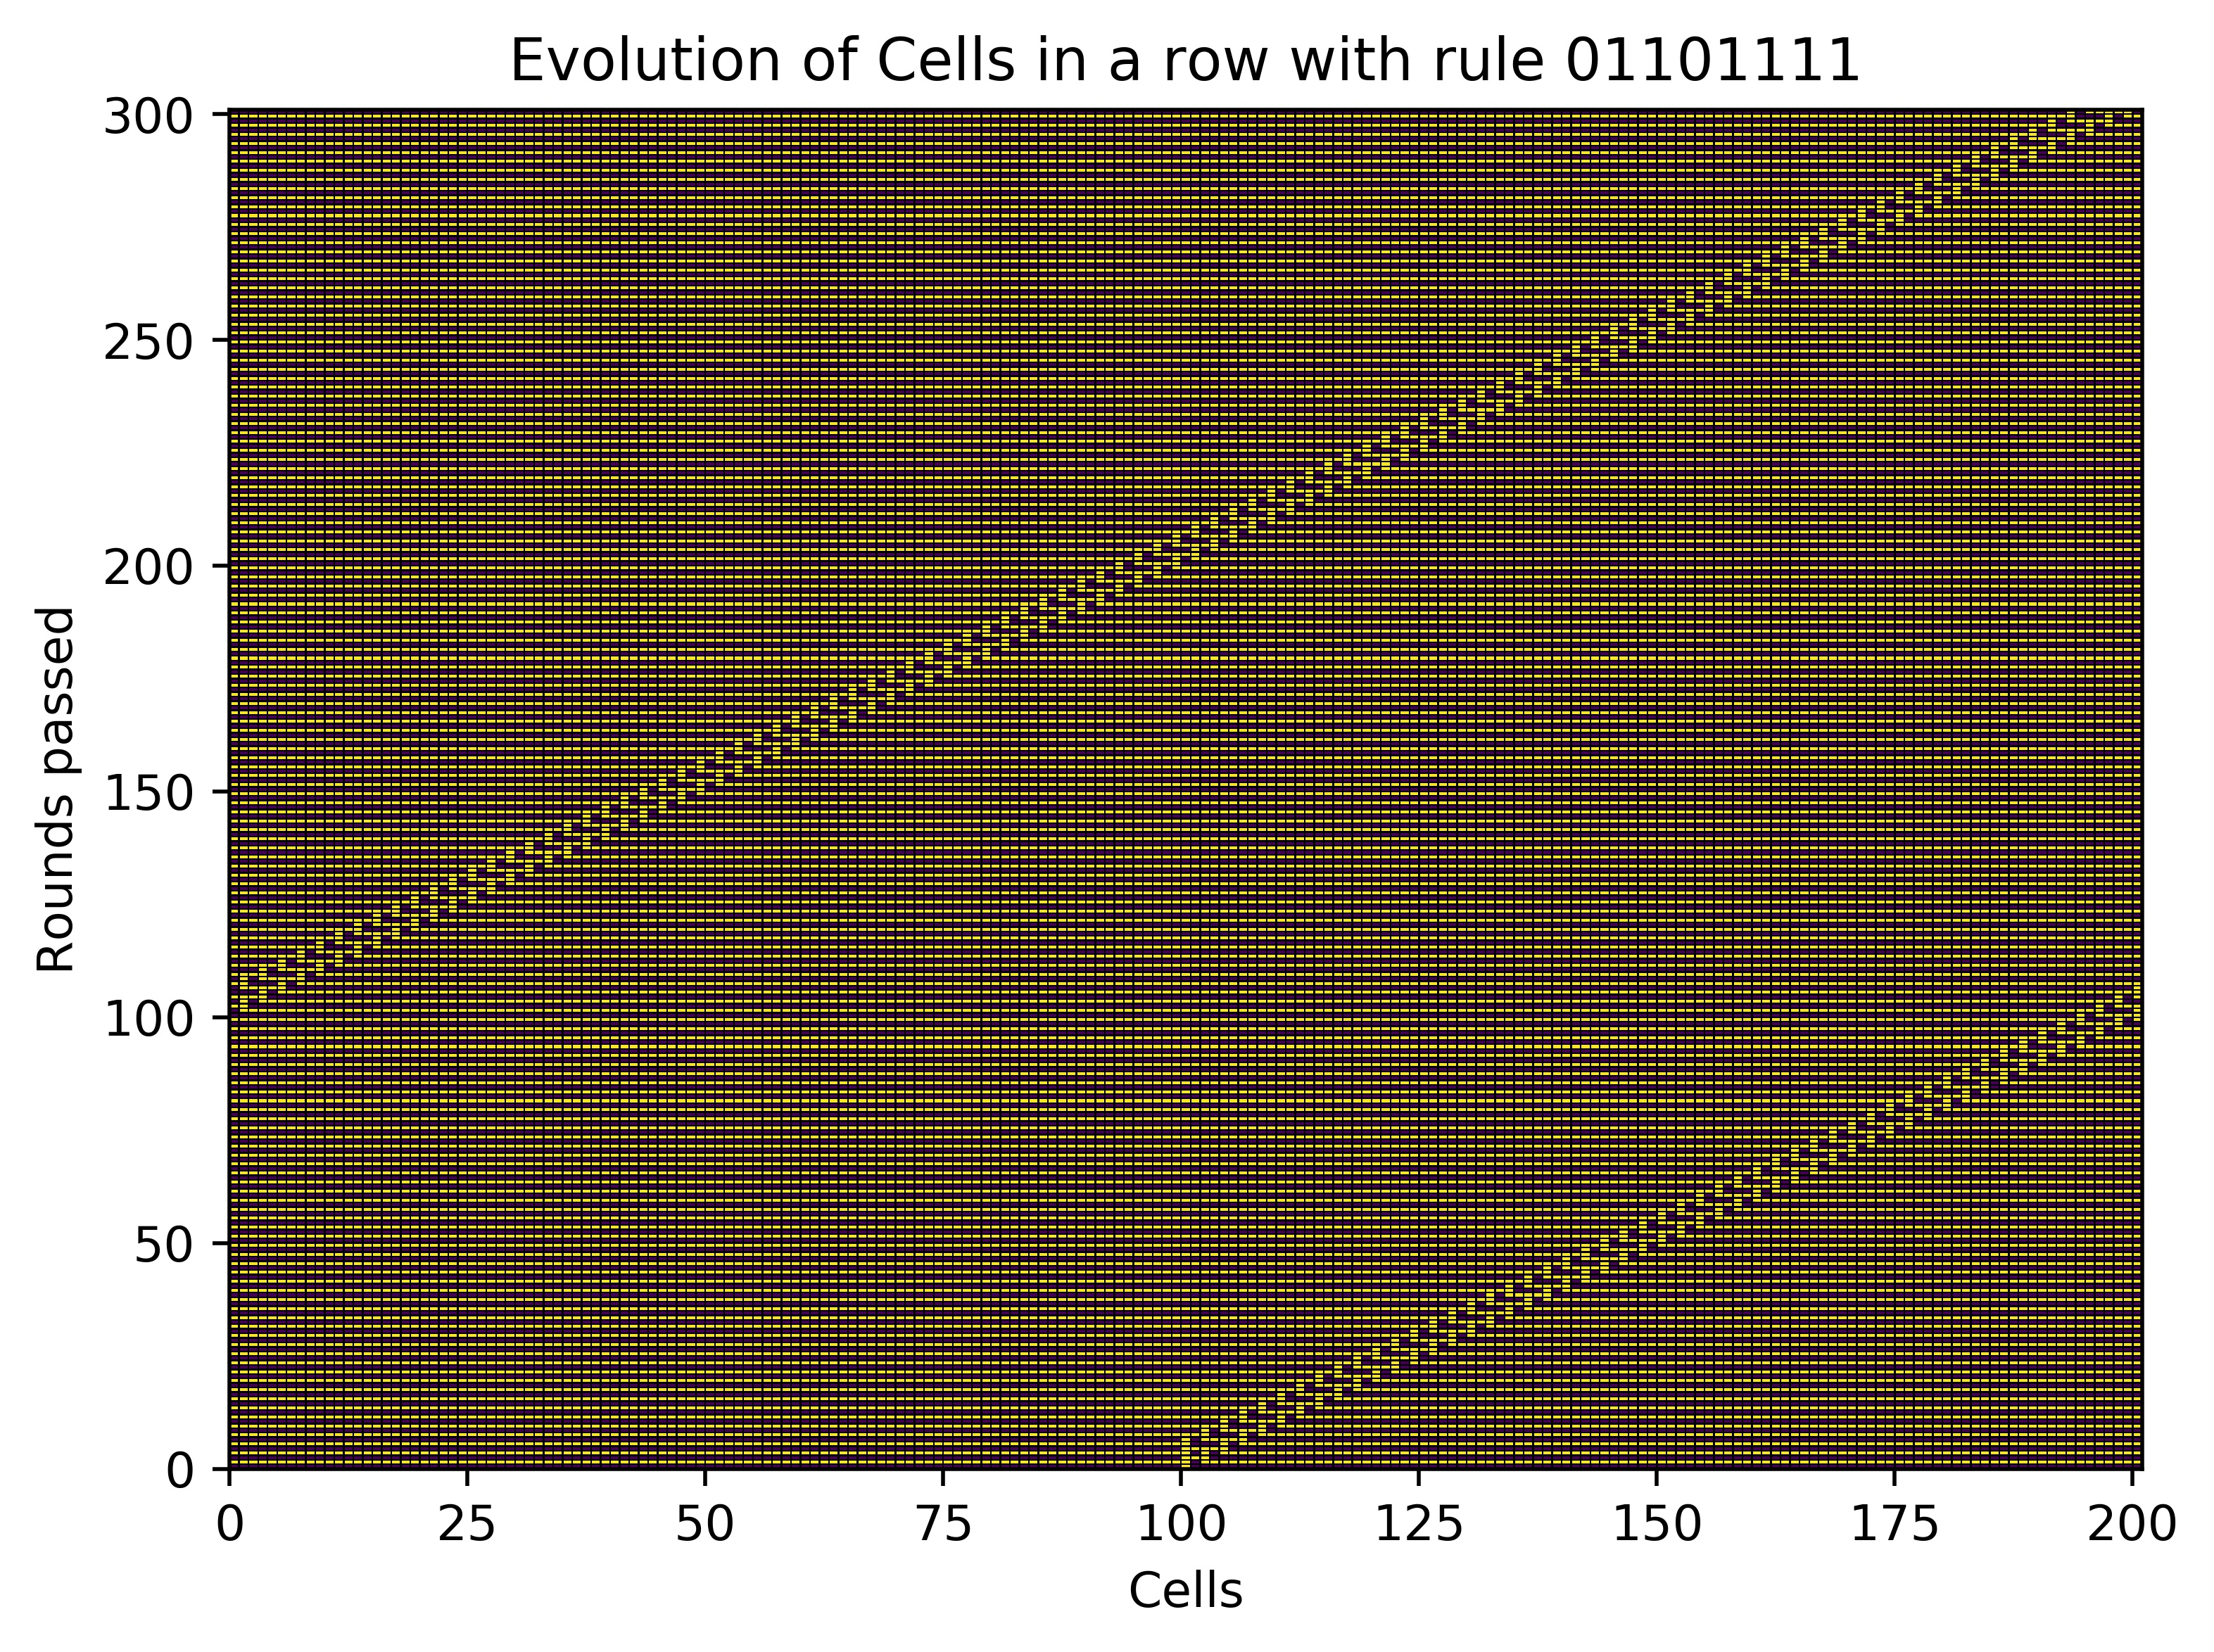
\includegraphics[width=0.4\linewidth]{../P3/Hats01101111.jpg}
		\includegraphics[width=0.4\linewidth]{../P3/Hats01111110.jpg}
		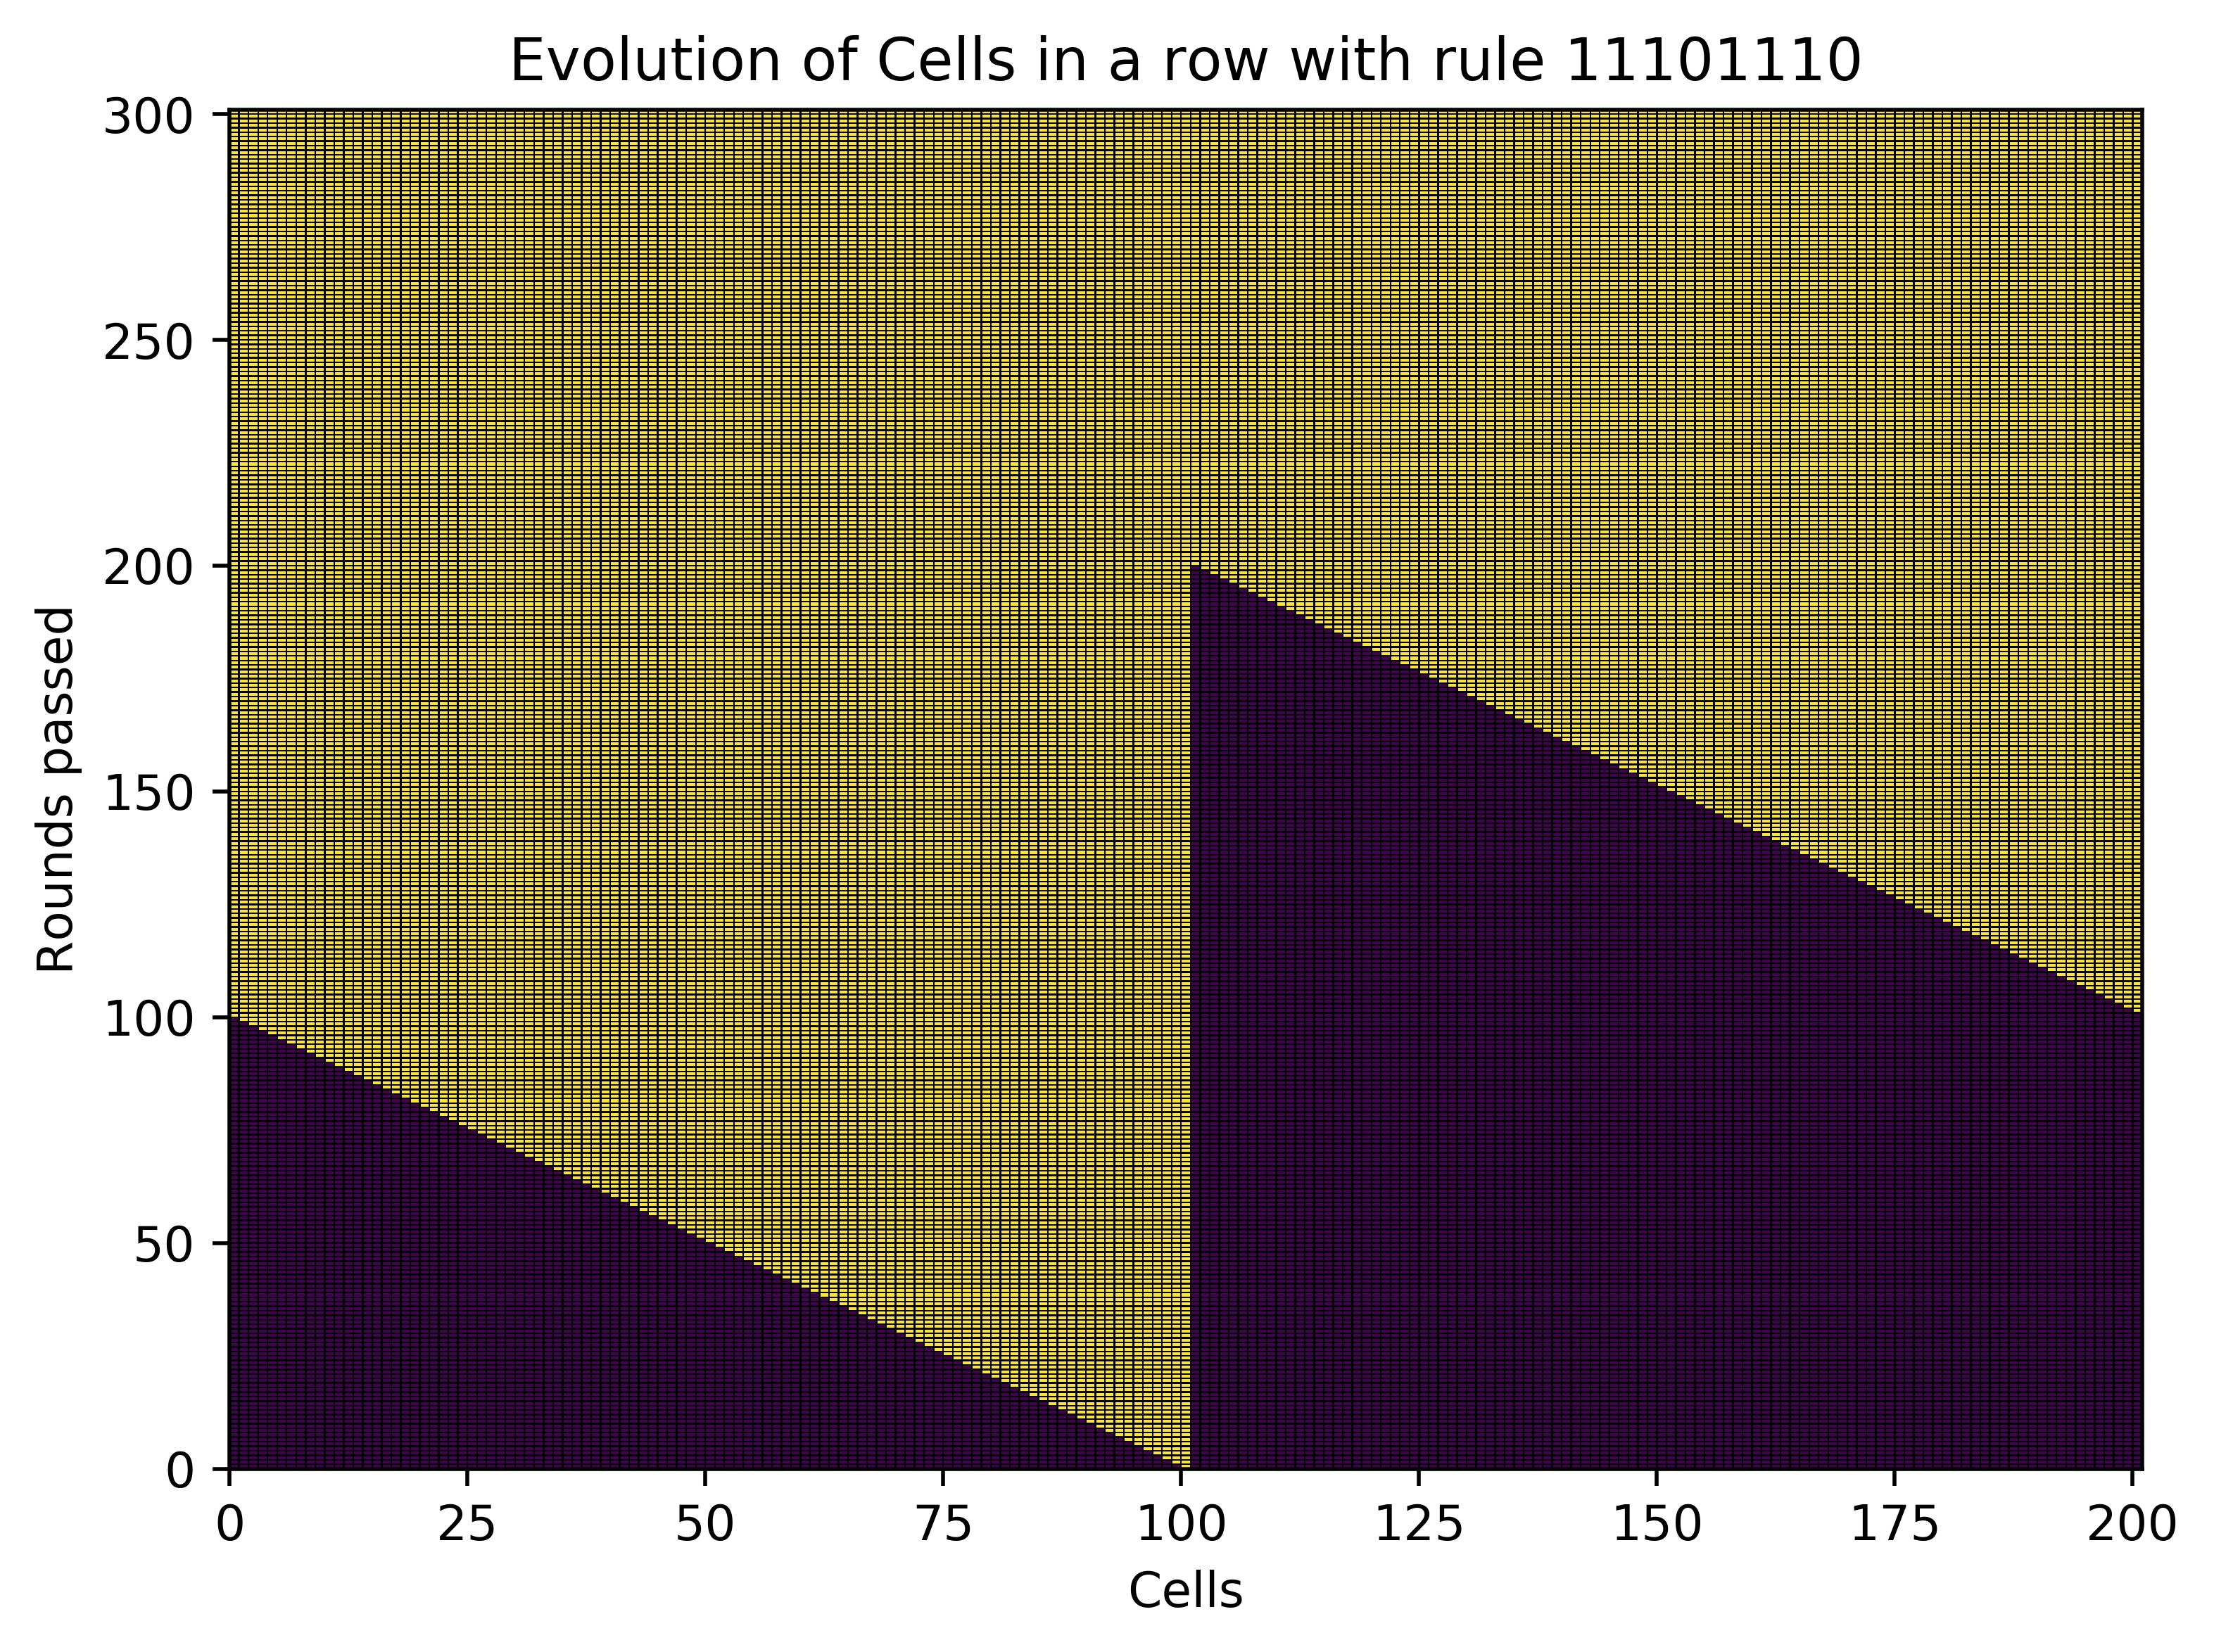
\includegraphics[width=0.4\linewidth]{../P3/Hats11101110.jpg}
		\label{fig:bitflip}
		\caption{This collections of images is created by performing bitflips on every binary
		digit of rule 110. The yellow cells are \emph{on} and the purple ones are \emph{off}.}
	\end{figure}
	
	\section{Problem 4}
	\subsection{The Code}
	Here we have the main file \texttt{gol.py} which stands for Game of Life (GoL).
	In the subfolder \texttt{classes}, we have \texttt{types.py} which contains a set initializers for our 4 models, \texttt{operations.py} which is contains everything
	we need to make decisions for the model, and \texttt{graphics.py} which consists of 
	the module \texttt{animate}. This module takes an array, makes a new one and initializes 
	it with the input, and prints an image of it. Then, it decides the next frame and saves the
	new array to \texttt{canvas}, and prints it, and so on the loop goes. I chose 20 frames to be the default. (Let's be honest, I just hard coded it! ;-P)
	\subsection{Results}
	At last, I took the frames and made a gif with them using \href{https://ezgif.com/maker}{this GIF Maker}. The files are available at the
	 corresponding subdirectories. I checked them with
	  \href{https://www.conwaylife.com/wiki/Main_Page}{this source} and 
	 they are spot on! Yay!
	 
	 
	 \section{Conclution}
	 I Hate \texttt{matplotlib.animation.FuncAnimation} soooo much!
	
	
\end{document}
